
%\subsection{Hydrate Complex Analysis}

%During the adsorption process of a gaseous \suldiox~moving in towards a water surface hydrate complexes are formed as the waters bind to the molecule. Computationally, there are various methods to determine hydrate complex formation. The most simple metric is to count the number of hydrogen bonds formed from the \suldiox~to neighboring molecules. This method can be furthered extended to also include the strength of those bonding interactions by additionally reporting the bondlengths to the hydrogen bonding partners. Longer bondlengths are typical of weaker bonds, and this method is used in this work to identify the bonding environment of the \suldiox~during solvation.

%A simple count of hydrogen bonds is telling of the interactions and environments of an adsorbing \suldiox. However, a more sophisticated analysis is needed to fully characterize the geometry of any complexes that form. In this work a graph theoretical method has been used to identify hydrate complexes that form cyclic structures in addition to those that form more simple hydrogen bonding geometries. Previously published works have detailed graph theory for use in molecular systems, and have used graph theoretical methods to describe ice and water clusters, structural energies, as well as in the study of relationships in biological systems.\cite{Huber2007,Shi2005,Radhakrishnan1991,Anick2002} As such, we will not present here a review of the basic graph theoretical details that are well documented in the referenced works. As shown in Figure \ref{fig:so2-complex-graph}, the atoms of a \suldiox~and its nearest neighbors are represented as a set of verrtices, with the covalent and hydrogen bonds between them forming the edges of a graph.

%We present here a technique for determining bonding cycles in a hydrate complex, but this technique is general enough to be applied to any graph representation of simple molecular systems. The first step in the determination of cycles is translating the atoms (vertices) and bonds (edges) to a graph. Figure \ref{fig:so2-complex-graph} shows the procedure visually, where here the root vertex of the graph is the \suldiox-sulfur, and each atom is numbered by the distance, in atoms, to the root vertex. We use only the closest neighboring water molecules that may take part in a cyclic complex in building the graph. After forming the graph, a breadth-first search (BFS) is performed starting at the root vertex.\cite{Knuth1997} The BFS algorithm uses a coloring technique where all unexamined vertices are colored white, queued vertices are gray, and examined vertices are black. During the BFS, encountering a gray vertex as a target of an adjacent edge during examination indicates that a cycle has been found in the graph. At each vertex dequeue for examination, the parent of every vertex is recorded such that the lineage from gray target to root vertex can be reconstructed to determine the participating atoms in the cycle.

%\begin{figure}[h!]
%\begin{center}
%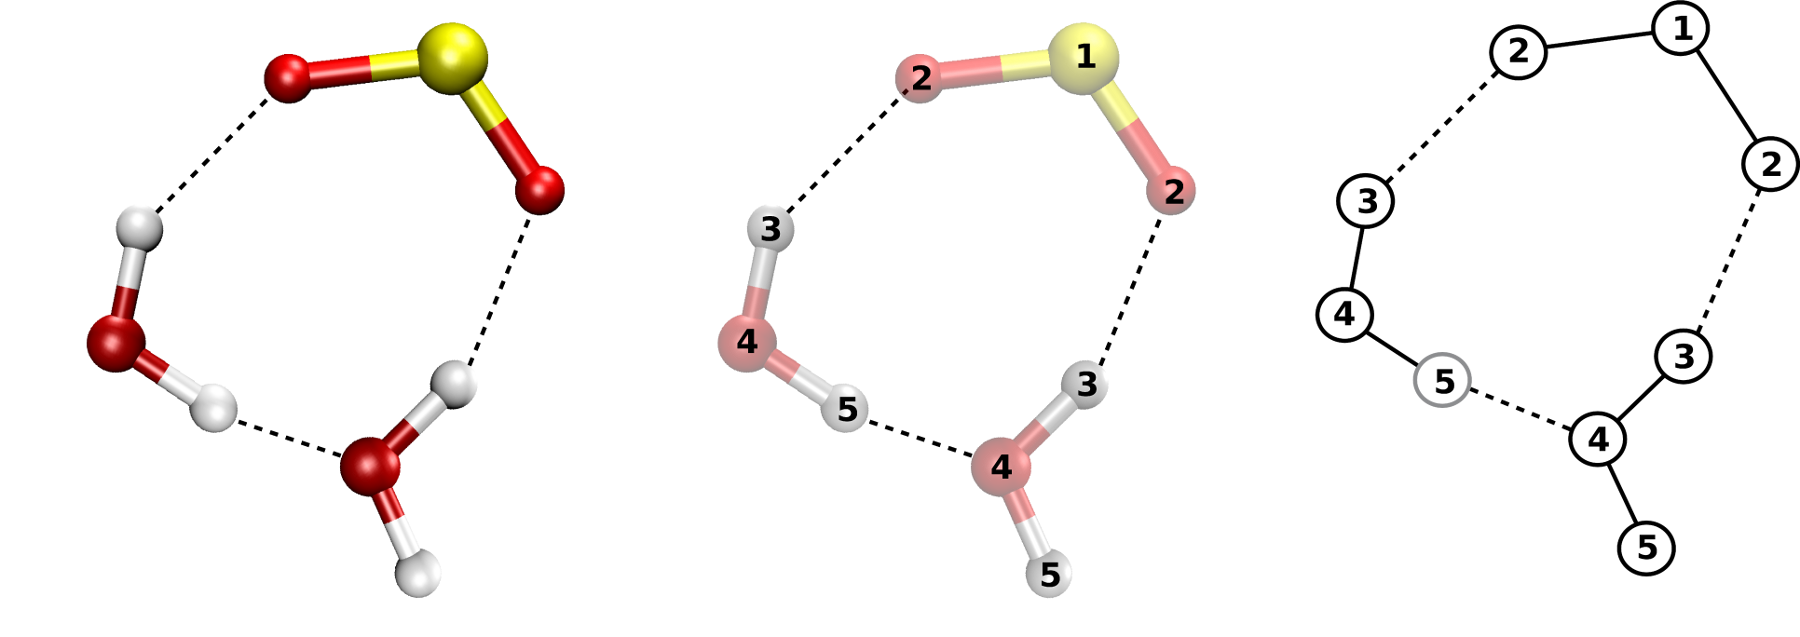
\includegraphics[scale=1.0]{images/Cycles/so2complexfigure.png}
%\caption{A \suldiox~and its nearest neighbors are represented as a graph of vertices and edges. The bonds are all given equal weights and the graph is undirected. The numbering shows the relative distance from any atom to the root node (\suldiox-sulfur 1), and also enumerates the iteration through the BFS process at which the atom is discovered. A BFS on this graph would result in discovering the doubly-bound hydrogen (5) as a gray target, and the gray source would be either of the connected oxygens (4). At each iteration the predecessor in the BFS is recorded in order to reconstruct the connectivity of the cycle. This cycle is composed of 8 atoms, and 3 molecules}
%\label{fig:so2-complex-graph}
%\end{center}
%\end{figure}
